\chapter{Deep Learning} \label{chap:basics-of-dl}

Deep learning is an area of machine learning that uses Artificial Neural Networks \parencite{mcculloch1943logical} and has been applied to a wide variety of tasks such as image classification, object recognition, activity recognition, 3D depth estimation, and various natural language processing (NLP) tasks. In stark contrast to the classical machine learning approach of designing manual feature extraction methods, deep learning focuses on creating algorithms that can automatically learn to extract relevant features.

\section{Deep Feedforward Networks} \label{sec:feed-forward-nets}

Deep feedforward networks, also called feedforward networks, or \textbf{multilayer perceptrons} (MLPs), are essential deep learning models. The goal of a feedforward network is to approximate some ideal function \(f^\star\). 
For example, a classifier \(y = f^\star(\symbfit{x})\) is a mapping between input $\symbfit{x}$ to a category $y$. A feedforward network has the ability to learn this mapping \(\symbfit{y} = f(\symbfit{x} \mathsemicolon \symbfit{\theta})\) where $\symbfit{\theta}$ is a set of learnt parameters that results in the best approximation of function $f^\star \approx f(\symbfit{x} \mathsemicolon \symbfit{\theta})$. In other words, neural networks (deep or otherwise) are function approximators.

These models are called \textbf{feedforward} because the information flows through the function that evaluates $\symbfit{x}$ and produces $\symbfit{y}$. The process of passing the input $\symbfit{x}$ through the function and through intermediate computations is known as \textbf{forward pass}.
We then use a \textbf{loss function} to measure the difference between $f^\star$ and $f$ - that is, the difference between the ideal mapping $f^\star$ and the estimated mapping $f$. 
The parameters of the network, $\symbfit{\theta}$, are updated in a \textbf{backward pass} based on some optimisation criteria, given the guidance of the loss function. 

% \includesvg{./assets/mlp.svg}
% \begin{figure}
%     \centering
%     % \captionsetup{justification=RaggedRight}
%     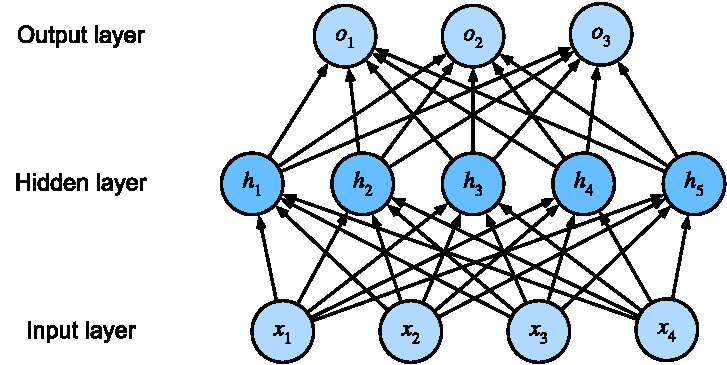
\includegraphics[scale=0.9]{chapters/assets/mlp.pdf}
%     \caption{An MLP with hidden layer consisting of $5$ hidden units. Image courtesy of \textcite{zhang2021dive}.}
%     \label{fig:mlp}
% \end{figure}
\def\layersep{2.5cm}
\begin{figure}
    \centering
    \captionsetup{justification=centering}
    \begin{tikzpicture}[shorten >=1pt,->,draw=black!50, node distance=\layersep]
    \tikzstyle{every pin edge}=[<-,shorten <=1pt]
    \tikzstyle{neuron}=[circle,fill=black!25,minimum size=17pt,inner sep=0pt]
    \tikzstyle{input neuron}=[neuron, fill=tudelft-green!50];
    \tikzstyle{output neuron}=[neuron, fill=tudelft-fuchsia!40];
    \tikzstyle{hidden neuron}=[neuron, fill=tudelft-cyan!50];
    \tikzstyle{annot} = [text width=4em, text centered]

    % Draw the input layer nodes
    \foreach \name / \y in {1,...,4}
    % This is the same as writing \foreach \name / \y in {1/1,2/2,3/3,4/4}
        \node[input neuron, pin=left:Input \#\y] (I-\name) at (0,-\y) {\(\symbfit{x}_{\y}\)};

    % Draw the hidden layer nodes
    \foreach \name / \y in {1,...,5}
        \path[yshift=0.5cm]
            node[hidden neuron] (H-\name) at (\layersep,-\y cm) {\(\symbfit{h}_{\y}\)};

    % Draw the output layer node
    \node[output neuron,pin={[pin edge={->}]right:Output}, right of=H-3] (O-0) {\(\symbfit{o}_{1}\)};
    \node[output neuron,pin={[pin edge={->}]right:Output}, right of=H-2] (O-1) {\(\symbfit{o}_{2}\)};
    \node[output neuron,pin={[pin edge={->}]right:Output}, right of=H-4] (O-2) {\(\symbfit{o}_{3}\)};

    % Connect every node in the input layer with every node in the
    % hidden layer.
    \foreach \source in {1,...,4}
        \foreach \dest in {1,...,5}
            \path (I-\source) edge (H-\dest);

    % Connect every node in the hidden layer with the output layer
    \foreach \source in {1,...,5}
        \foreach \dest in {0,...,2}
            \path (H-\source) edge (O-\dest);

    % Annotate the layers
    \node[annot,above of=H-1, node distance=1cm] (hl) {Hidden layer};
    \node[annot,left of=hl] {Input layer};
    \node[annot,right of=hl] {Output layer};
\end{tikzpicture}
    \caption{An MLP with a hidden layer consisting of $5$ hidden units.}
    \label{fig:mlp}
\end{figure}

Feedforward neural networks are called \textit{networks} because they are typically composed of many different functions. The model is associated with a directed acyclic graph that describes how the functions are composed together.
For example, we can have three functions \(f^{(1)}, f^{(2)}\) and $f^{(3)}$ connected in a chain, to form \(f = f^{(1)} \circ f^{(2)} \circ f^{(3)}\). 
Chain structures such as these are quite commonly used structures of neural networks. Here, $f^{(1)}$ is the \textbf{first layer}, $f^{(2)}$ is the \textbf{second layer} and so on. 
The final layer is called \textbf{output layer}, in this small example, $f^{(3)}$ is the output layer. The training data or training strategy determines what the output layer must produce for each given input $\symbfit{x}$.
Intermediate layers such as $f^{(2)}$ that do not directly produce the output $\symbfit{y}$ are called \textbf{hidden layers}.

Each hidden layer of the network is typically vector valued. The dimensionality of these hidden layers determines \textbf{width} of the model. Each element in the vector plays a role analogous to a neuron. Instead of thinking of a layer as a vector-to-vector function, we can also think of the layer as consisting of many \textbf{units} that act in parallel \parencite{Pinker1988}, each representing a vector-to-scalar function. 
\Cref{fig:mlp} shows a small MLP with a single hidden layer. Each of the nodes in \cref{fig:mlp} represents a value in a vector; this implies that the input $\symbfit{x}$ has a dimensionality of $4$, the hidden layer (intermediate values) has a dimensionality of $5$ and the output has a dimensionality of $3$.

Now, we must choose the form of our model, $f(\symbfit{x} \mathsemicolon \symbfit{\theta})$. Let us choose a linear model parameterised by $\symbfit{\theta}$ consisting of $\symbfit{w}$ and $b$, where $\symbfit{w}$ provides the weights and $b$ provides the biases (or intercepts):
\begin{equation}
    \label{eqn:linear-model}
    f(\symbfit{x}; \symbfit{\theta}) = f(\symbfit{x} ; \symbfit{w}, b)=\symbfit{x}^{\top} \symbfit{w} + b.
\end{equation}

For the model in \cref{fig:mlp} whose hidden layer has $\symbfit{h}$ units, which are calculated by a function \(f^{(1)}(\symbfit{x}; \symbfit{W}, \symbfit{c})\) that is linear similar to the form of \cref{eqn:linear-model}. 
The values of these hidden units are then used as input to the second layer, which is also the output layer of the network. The output layer is also a linear function applied to $\symbfit{h}$ rather than to $\symbfit{x}$.
The network now has two functions chained together \(\symbfit{h} = f^{(1)}(\symbfit{x}; \symbfit{W}, \symbfit{c})\) and \(y = f(\symbfit{h} ; \symbfit{w}, b)\), with the complete model being $f(\symbfit{x} ; \symbfit{W}, \symbfit{c}, \symbfit{w}, b)=f^{(2)}\left(f^{(1)}(\symbfit{x})\right)$. It should be noted that a model parameterised by $\symbfit{\theta}$ implies that $\symbfit{\theta}$ is a collection of all the weights and biases present in the network.

Unfortunately, the complete model $f$ is a linear function of its input, since we have chosen both $f^{(1)}$ and $f^{(2)}$ to be linear. 
However, not all data spaces are linear. More often than not, they are non-linear in nature; accordingly, we must introduce a non-linear function to describe the data and its features.
Most neural networks do so using an \textbf{affine transformation} controlled by the learned parameters (such as $\symbfit{\theta}$), followed by a fixed nonlinear function called an \textbf{activation function}.

\section{Activation Functions} \label{sec:activation-functions}

Activation functions decide whether or not a neuron (node in \cref{fig:mlp}) should be activated. More specifically, they are differentiable operators to transform inputs to outputs and add some form of non-linearity in the transformation. Formally, our hidden-layer output is now defined as:
% \begin{equation}
%     f(\symbfit{x}; \symbfit{\theta}) = f(\symbfit{x}; \symbfit{w}, b) = g(\symbfit{x}^\top\symbfit{w} + b)
% \end{equation}
\begin{equation}
\begin{split}
    \symbfit{h} &= g \circ f^{(1)} \left(\symbfit{x}\right)\\
                &=g\left(\symbfit{W}^{\top} \symbfit{x}+\symbfit{c}\right)
\end{split}
\end{equation}
where $\symbfit{W}$ is the linear transformation, $\symbfit{c}$ the biases and $g(\cdot)$ is an \textbf{activation function} whose job is to introduce some non-linearity. Previously, we had used a vector of weights and a scalar bias parameter in \cref{eqn:linear-model} to describe an affine transformation from a vector input to a scalar output. However, now we are describing an affine transformation from a vector $\symbfit{x}$ to a vector $\symbfit{h}$, so an entire vector of biases is needed.

One of the most widely used activation functions is \textbf{ReLU} (Rectified Linear Unit) \parencite{Fukushima1975}. This function simply returns the maximum between the given input value and zero, as given in \cref{eqn:relu}. As such, this simple function has a minimal computation cost and can be performed quite quickly.
\begin{equation}\label{eqn:relu}
    \begin{split}
        g \circ f(\symbfit{x}) & = \operatorname{max}\left(0, f^{(1)}(\symbfit{x})\right)\\
                               & = \operatorname{max}\left(0, \symbfit{W}^\top\symbfit{x} + \symbfit{c}\right)
    \end{split}
\end{equation}

Another important and common function is the \textbf{Sigmoid} \cref{eqn:sigmoid} function. This function maps the input value to a real number between $(0, 1)$.
In earlier forms of nerural networks \parencite{mcculloch1943logical}, scientists where interested in neurons that either fire or do not, and so used thresholding units. A thresholding activation takes value $0$ when its input is below a certain threshold and takes value $1$ if its input is higher than the threshold. 
Sigmoids, on the other hand, are smooth and differentiable approximations of thresholding units; this is favourable to the gradient-based learning adopted in today's time.
Sigmoids are used largely in output units when we want to interpret the output as probabilities for binary classification problems.
\begin{equation}\label{eqn:sigmoid}
    \begin{split}
        \operatorname{sigmoid}(\symbfit{x}) = \sigma(\symbfit{x}) & = \frac{1}{1 + \exp(-\symbfit{x})}.
        % \operatorname{sigmoid}(\symbfit{h}) & = \frac{1}{1 + \exp(-(\symbfit{W}^\top\symbfit{x}+\symbfit{c}))}.
    \end{split}
\end{equation}

Like the sigmoid function, the \textbf{tanh} (hyperbolic tan) function also squashes its inputs, mapping them between $-1$ and $1$:
\begin{equation}
\begin{split}
    \operatorname{tanh}(\symbfit{x}) & = \frac{1 - \exp(-2\symbfit{x})}{1 + \exp(-2\symbfit{x})}.
    % \operatorname{tanh}(\symbfit{h}) & = \frac{1 - \exp(-2(\symbfit{W}^\top\symbfit{x}+\symbfit{c}))}{1 + \exp(-2(\symbfit{W}^\top\symbfit{x}+\symbfit{c}))}.
\end{split}
\end{equation}

\begin{figure}[t]
     \centering
     \captionsetup{justification=centering}
     \begin{subfigure}[b]{0.3\textwidth}
         \centering
         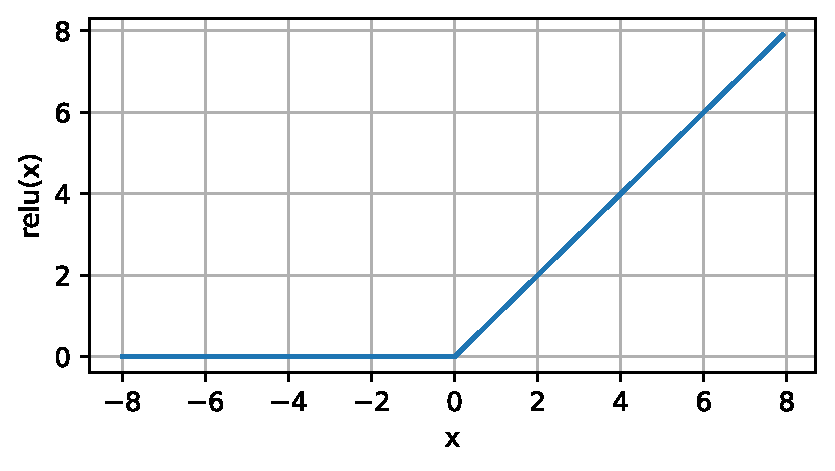
\includegraphics[width=\textwidth]{chapters/assets/relu.pdf}
         \caption{ReLU}
         \label{fig:relu}
     \end{subfigure}
     \hfill
     \begin{subfigure}[b]{0.3\textwidth}
         \centering
         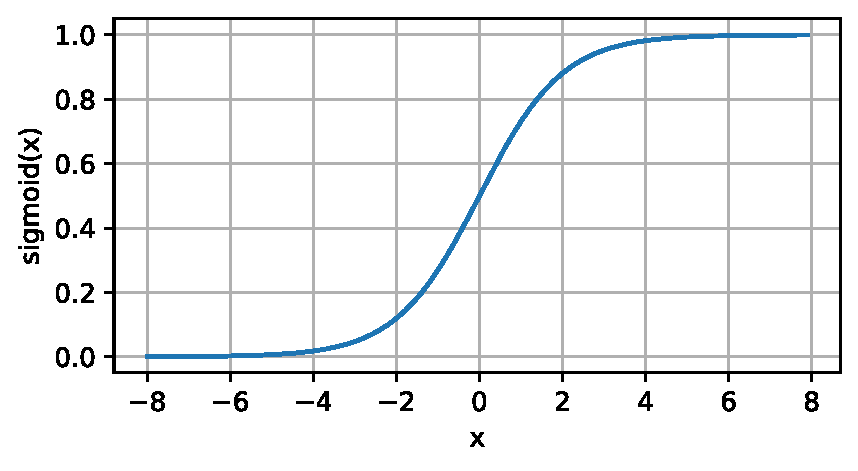
\includegraphics[width=\textwidth]{chapters/assets/sigmoid.pdf}
         \caption{Sigmoid}
         \label{fig:sigmoid}
     \end{subfigure}
     \hfill
     \begin{subfigure}[b]{0.3\textwidth}
         \centering
         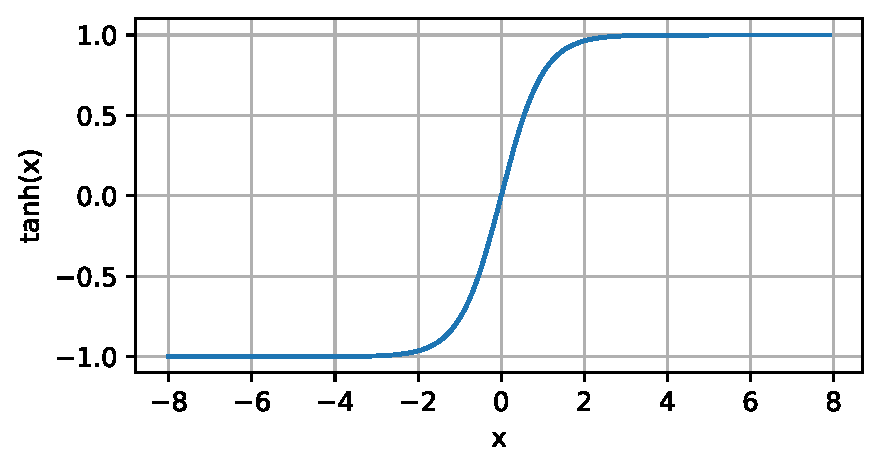
\includegraphics[width=\textwidth]{chapters/assets/tanh.pdf}
         \caption{Tanh}
         \label{fig:tanh}
     \end{subfigure}
        \caption{Three common activation functions.}
        \label{fig:three-activation-funcs}
\end{figure}

\section{Loss Function}\label{sec:loss-fn}
During training, for each training sample in the training set $\{\symbfit{x}_i, y_i\}_{i=1}^m$ where $\symbfit{x}_i$ is an input vector and $y_i$ is the corresponding label, we present the input $\symbfit{x}$ to the neural network and compare the predicted output of the network $\hat{y}_i$ with the corresponding label $y_i$.
We need to define a \textbf{loss function} to objectively measure how much the predicted output of the network $\hat{y}_i$ is different from the expected output $y_i$. For regression problems, the quadratic loss function called the mean squared error (MSE) is calculated as follows:
\begin{equation}
    \mathcal{L}(\symbfit{\hat{y}}, \symbfit{y}) = \frac{1}{2} \| \symbfit{y} - \symbfit{\hat{y}} \| ^ 2
\end{equation}

The loss function is calculated for each training example in the training set. The average of the calculated loss functions for all training examples in the training set is called the \textbf{cost function}. For MSE it is the average of the calculated loss functions for all training examples in the training set:
\begin{equation}
    J(\symbfit{\theta}) = \frac{1}{2m} \sum_{j=1}^{m} \| \symbfit{y}_i - \symbfit{\hat{y}_i} \| ^ 2
\end{equation}
where $m$ is the total number of training samples. In the following \Cref{sec:softmax} we shall see another loss function that is important for multiclass classification.

\section{Softmax} \label{sec:softmax}
For convenience in the following section, we shall call the network output $f(\symbfit{x}; \symbfit{\theta})$ as $\symbfit{o}$. Assume that we have a loss function such as mean squared error loss (MSE). When working with \textbf{multiclass classification} problems, where \(\symbfit{y} \in \left\{1,\ldots, K \right\}\); we expect the output of the model to be a vector of class probabilities where each value tells us the probability that a sample belongs to a particular class.
Note that we generally employ the ``one-hot'' encoding mechanism where $\symbfit{y} = (0, ... , 0, 1, 0, ... , 0)$.
We can try to directly minimise the difference between $\symbfit{o}$ and $\symbfit{y}$. Although treating classification as a regression problem may work well, it still lacks in two main ways:
\begin{itemize}
    \item There is no guarantee that $\symbfit{o}$ will sum up to $1$ as we have come to expect from probabilities
    \item There is no guarantee that $\symbfit{o}$ takes strictly non-negative values regardless of the sum of $\symbfit{o}$
\end{itemize}

Both of these issues make the problem difficult to solve in addition to making the solution highly sensitive to outliers. If we were to presume a positive linear dependency between the horsepower of a car and the probability that someone will buy it, the probability might exceed $1$ when it comes to buying a Bugatti Chiron\footnote{\url{https://www.bugatti.com/models/chiron-models/}}! Of course, this breaks the mathematical and logical rules of probability theory; therefore, we need a technique to map the values of $\symbfit{o}$ between $(0, 1)$.
% TODO: should we talk about data generating distribution here?

One way to accomplish these goals (ensuring that the output sums up to $1$ and its values are non-negative), is to use an exponential function $P(y = i) \propto \exp o_i$. The $\exp$ function does ensure that the output will always be non-negative. We can further \textbf{normalise} these values so that they add up to $1$ by dividing each by the sum of the whole. This gives us the \textbf{softmax} function:
\begin{equation}
    \hat{\symbfit{y}} = \operatorname{softmax}(\symbfit{o}) \quad \text{where}\quad \hat{y}_i = \frac{\exp(o_i)}{\sum_{j=1}^{K} \exp(o_j)}.
    \label{eqn:std-softmax}
\end{equation}

Note that the highest value in $\symbfit{o}$ corresponds to the most likely class according to $\symbfit{\hat{y}}$. Softmax also preserves the ordering of its arguments as shown in the example:
\begin{equation}
    \nonumber
    \operatorname{softmax} \left(\begin{bmatrix}
    8\\
    5\\
    0
    \end{bmatrix}\right)
    = 
    \begin{bmatrix}
    0.9523\\
    0.0474\\
    0
    \end{bmatrix}.
\end{equation}

\subsection{Softmax and Cross-Entropy Loss}\label{ssec:ce-loss}

The softmax function gives us a vector $\symbfit{\hat{y}}$, which we can interpret as (estimated) conditional probabilities of each class, given any input $\symbfit{x}$, like $P(y=\text{class} | \symbfit{x})$. 
The cross-entropy loss measures the difference between two probability distributions; in this case, it measures the difference between $\symbfit{\hat{y}}$ and $\symbfit{y}$. The cross-entropy loss is given as:
\begin{equation}\label{eqn:ce-loss}
    \mathcal{L}(\symbfit{y}, \hat{\symbfit{y}}) = - \sum_{j=1}^K y_j \log \hat{y}_j.
\end{equation}

Note that the loss defined in \cref{eqn:ce-loss}, has a lower bound of $0$ when $\hat{\symbfit{y}}$ is a probability vector, that is, no single entry is greater than $1$, and hence its negative logarithm cannot be lower than $0$. For multiclass classification problems, the cost function is calculated as follows:
\begin{equation}
    J(\symbfit{\theta}) = - \frac{1}{m} \sum_{j=1}^{m} \sum_{i=1}^{c} \symbfit{y_{i}^{(j)}}\log(\symbfit{\hat{y}_{i}^{(j)}})
\end{equation}

To better understand the origins of the cross-entropy loss, please refer to \textcite{zhang2021dive}.

\subsection{Softmax vs Sigmoid}\label{ssec:softmax-vs-sigmoid}
The softmax and sigmoid functions are similar, as they help squeeze the network output within a certain range. The softmax function operates on a vector input, while the sigmoid takes a scalar value as input. In fact, the sigmoid function is a special case of the softmax function for a classifier with only two input classes (binary classification problem). We can show this if we set the input vector to $\symbfit{z} = [x, 0]$ and calculate the first output element with the usual softmax formula:
\begin{align*}
    \operatorname{softmax}(\symbfit{z})_{1}&=\frac{\exp{(z_{1})}}{\exp{(z_{1})}+\exp(z_{2})} \\
    &= \frac{\exp(x)}{\exp(x)+\exp(0)} \\
    &= \frac{\exp(x)}{\exp(x)+1} && \text{divide numerator and denominator by} \exp{(x)}\\
    &= \frac{1}{1 + \exp(-x)}
\end{align*}


\section{Universal Approximation Theory}\label{sec:uat}

MLPs are of extreme importance in deep learning, as they form the basis for many applications and advanced neural architectures. To do this, MLPs and neural networks, in general, must be able to approximate a wide range of functions, given enough input data to learn from. Neural networks started as a way to mimic the neural structure of the brain \parencite{mcculloch1943logical}, and as we know our brain is capable of complex statistical analysis, among other things. As such, a worthwhile question to ask here is \textit{just how powerful can a deep neural network be?}
Fortunately for us, this question has been answered several times in the context of MLPs and radial basis functions (RBF) \parencite{Cybenko1989, Micchelli1986, Hornik1991}. These works suggest that even with a single hidden layer, given enough nodes and the right set of parameters $\symbfit{\theta}$, we can potentially model any function. 
In simple terms, having enough nodes and stacking enough affine transformations followed by non-linear transforms repetitively, a neural network should be able to model a highly rich class of functions.
Although neural networks are capable of expressing arbitrary continuous functions, it may not be easy to learn the function and its parameters.

\section{Optimisation and Backpropagation}\label{sec:optimisation}

Until now, we have only discussed the forward pass of a neural network, where the network processes the input $\symbfit{x}$. However, to effectively approximate $f^\star$, a neural network must learn an ideal set of values for the parameters, $\symbfit{\theta}$. To do so, we must \textbf{optimise} the weights so that they are suitable for the task and the data at hand. However, the optimisation algorithms used to train deep learning models differ from traditional optimisation algorithms in multiple ways. In most machine tasks, we are concerned with some performance measure $P$, which is defined with respect to the test set and may very well be intractable. Therefore, we optimise $P$ indirectly through a cost function $J\symbfit{(\theta)}$.

Typically, the cost function is written as an average over the training set (see \Cref{sec:loss-fn}):
\begin{equation}
\label{eqn:cost-fn-emp}
\begin{split}
    J(\symbfit{\theta})&=\mathbb{E}_{(\symbfit{x}, \mathrm{y}) \sim \hat{p}_{\mathrm{data}}} \mathcal{L}(f(\symbfit{x} ; \symbfit{\theta}), y)\\
    &= \mathbb{E}_{(\symbfit{x}, \mathrm{y}) \sim \hat{p}_{\mathrm{data}}} \mathcal{L}(\hat{y}, y)
\end{split}
\end{equation}
where $\mathcal L$ is the loss function per sample, $\hat{y} = f(\symbfit{x}; \symbfit{\theta})$ is the predicted output, the input is $\symbfit{x}$ and \(\hat{p}_{\mathrm{data}}\) is the empirical (observed) distribution. In the straightforward supervised case, $y$ is the true target output. It takes minimal effort to adapt this formulation to exclude $y$ as an argument, as we shall see this in \Cref{chap:self-supervised-learning}.


\subsection{Gradient Descent}\label{sec:sgd}

We begin by assuming that we have a function $y = f(x)$ where $x, y \in \mathbb{R}$ and that it has a derivative $f^\prime(x)$. The derivative of a function gives its slope, also called \textbf{gradient} at a certain input point $x$. The gradient indicates how adding a small change $\epsilon$ to $x$ will affect the output: $f(x + \epsilon) \approx f(x) + \epsilon f^\prime(x)$. Gradient descent is a first-order iterative optimisation algorithm used to find the local minimum or maximum of a function \parencite{Kiefer1952, Robbins1951}. The optimisation algorithm works by iteratively moving in the direction of steepest descent, as defined by the negative of the gradient.

\begin{figure}[ht]
    \centering
    \captionsetup{justification=RaggedRight}
    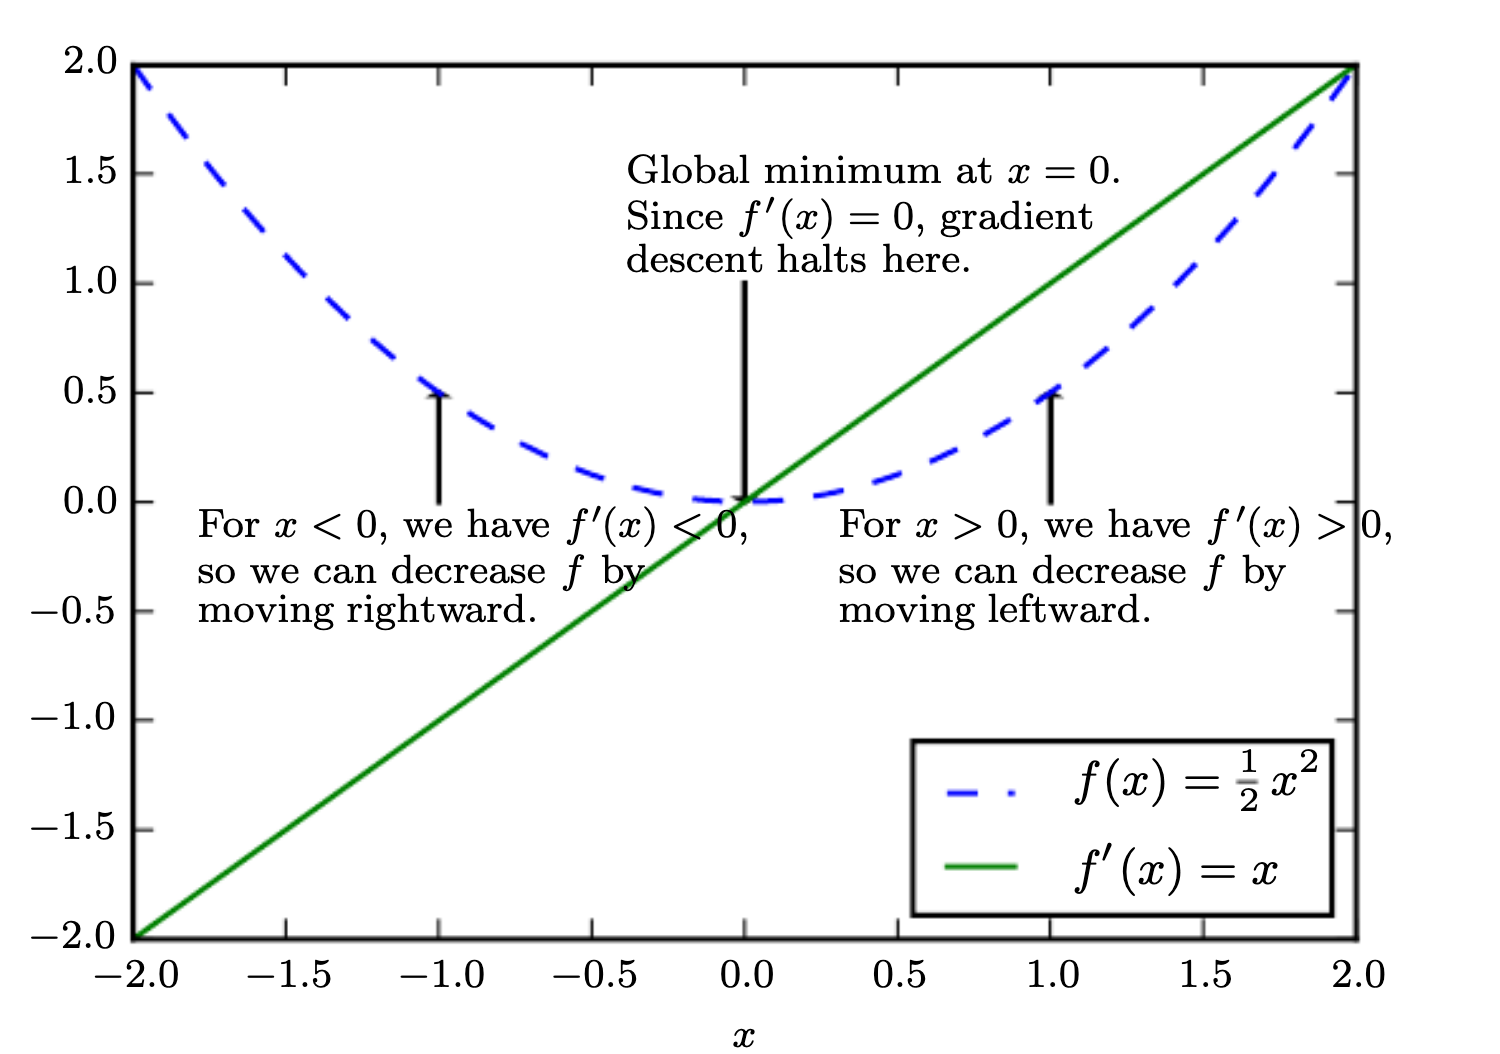
\includegraphics[scale=0.15]{chapters/assets/gradient_descent_basic.png}
    \caption{Gradient descent algorithm illustration for finding the minimum of a function $f(x) = \frac{1}{2}x^2$. Beginning with either positive of negative values of $x$, the gradient descent algorithm will find a minima at $x=0$ by moving in the direction opposite the sign of the gradient given by $f^\prime(x)=x$. Figure courtesy of \textcite{GoodfellowDLBook2016}.}
    \label{fig:gradient-descent}
\end{figure}

In \cref{fig:gradient-descent} the function $f(x)=\frac{1}{2}x^2$ depends only on the input $x$ and has a derivative \(f^\prime(x)=x\). In order to find the minimum of $f(x)$ we must find the value of $x$ where $f^\prime(x)=0$. The useful property of the gradient is that it tells us how to change $x$ to make a small change to $y$. For instance, we can infer that $f\left(x-\epsilon \operatorname{sign}\left(f^{\prime}(x)\right)\right) \ll f(x)$ for a small $\epsilon$. 
Therefore, to reduce $f(x)$, we can begin this process by starting with positive or negative values of $x$ and moving in the direction opposite to the sign of the gradient $f^\prime(x)$. The process is known as \textbf{gradient descent}, more specifically this update step reads:
\begin{align}
    x^\prime &=x-\epsilon \operatorname{sign}\left(f^{\prime}(x)\right) \nonumber \\
    &= x-\epsilon \operatorname{sign}\nabla_x f(x) \quad
\end{align}

\subsection{Backpropagation}\label{eqn:backprop}
The backpropagation as a learning algorithm was put forth by \textcite{rumelhart1986learning}, and is firmly based on the concept of gradient descent. We discussed gradient descent in the context of a simple function $f(x)$ that was dependent only on its input $x$, however, neural networks depend on the input $\symbfit{x}$ and a set of parameters $\symbfit{\theta}$, $f(\symbfit{x} \mathsemicolon \symbfit{\theta})$. Furthermore, the learning goal of neural networks is not to directly minimise the function $f(\symbfit{x} \mathsemicolon \symbfit{\theta})$. Rather, the goal of learning in neural networks is to minimise the cost function (or loss function) given the training set. 

Consider a network parameterised by $\symbfit{\theta} = \{\symbfit{w}, b\}$. The goal of backpropagation is to calculate partial derivatives \(\sfrac{\partial J}{\partial \symbfit{w}}\) and \(\sfrac{\partial J}{\partial b}\) of the cost function $J$ with respect to weight $\symbfit{w}$ and bias $b$. To further concretize the notion, we shall use the MSE loss from \Cref{sec:loss-fn}:
\begin{align}
    \mathcal{L}(\symbfit{\hat{y}}, \symbfit{y}) &= \frac{1}{2} \| \symbfit{y} - \symbfit{\hat{y}} \| ^ 2 \\
    J(\symbfit{\theta}) &= \frac{1}{2N} \sum_{i=1}^{N} \mathcal{L}(f(\symbfit{x} \mathsemicolon \symbfit{\theta}), \symbfit{y})
    \label{eqn:bp-cost-fn}
\end{align}
where $N$ is the total number of training samples. To calculate \(\sfrac{\partial J}{\partial \symbfit{w}}\) and \(\sfrac{\partial J}{\partial b}\), we apply the \textbf{chain rule} and calculate, in turn, the gradient of each intermediate variable and parameter. The first step is to calculate $\sfrac{\partial J}{\partial \mathcal{L}}$ which are the gradients of the cost function in \Cref{eqn:bp-cost-fn} with respect to the loss term $\mathcal{L}$.
Next, we must compute the gradient of the cost function with respect to the output variable $\symbfit{\hat{y}}$ according to the chain rule:
\begin{equation}
    \frac{\partial J}{\partial \symbfit{\hat{y}}}
= \frac{\partial J}{\partial \mathcal{L}} \times \frac{\partial \mathcal{L}}{\partial \symbfit{\hat{y}}}.
\end{equation}
Now we can calculate the gradient \(\sfrac{\partial J}{\partial \symbfit{w}}\), using the chain rule this yields:
\begin{equation}
    \frac{\partial J}{\partial \symbfit{w}}= \left(\frac{\partial J}{\partial \symbfit{\hat{y}}} \times \frac{\partial \symbfit{\hat{y}}}{\partial \symbfit{w}}\right).
\end{equation}
where \(\sfrac{\partial \symbfit{\hat{y}}}{\partial \symbfit{w}} = \symbfit{x}\).

Notice that the order of calculations are now \textbf{reversed} relative to those performed in the forward pass. Here we start with the output emitted by the neural network and work our way backwards towards the parameters. We can repeat the above steps for computing \(\sfrac{\partial J}{\partial b}\). Intuitively, this tells us how to update $\symbfit{w}$ and $b$ in order to reduce $J(\symbfit{\theta})$.

We must also be aware of the fact that we optimise for the loss function $\mathcal{L}$, that is, we are trying to find the optimal set of parameters $\symbfit{\theta}$ that will give us the lowest value of the loss function across $N$ training samples. In other words, we are trying to find the minima of $\mathcal L$ with respect to the input $\symbfit x$ and the parameters $\symbfit{\theta}$.
The gradient $\nabla_{\symbfit{\theta}}J$ across all samples is given as:
\begin{equation}
    \nabla_{\theta} J(\symbfit{\theta}) = \frac{1}{2N} \sum_{i=1}^{N}\nabla_{\symbfit{\theta}}\mathcal{L}(f(\symbfit{x};\symbfit{\theta}), y)
    % \bigg[\frac{\partial L}{\partial w}, \frac{\partial L}{\partial b}, \ldots \bigg]^\top
\end{equation}
where $\nabla_{\theta} J(\symbfit{\theta})$ is the average of the gradients of the loss function with respect to $\symbfit x$ and $\symbfit{\theta}$. The parameter update using the gradient descent algorithm with step size $\eta$ can be written as
\begin{equation}
    \label{eqn:basic-gd}
    \symbfit{\theta}^\prime=\symbfit{\theta}-\eta \nabla_{\theta} J(\symbfit{\theta}).
\end{equation}

However, this method is intractable for very large values of $N$. Therefore, we choose to compute gradients for a smaller set of $m$ samples such that $m \ll N$:
\begin{equation}
    \nabla_{\theta} J(\symbfit{\theta}) = \frac{1}{2m} \sum_{i=1}^{m}\nabla_{\symbfit{\theta}}\mathcal{L}(f(\symbfit{x};\symbfit{\theta}), y).
    % \bigg[\frac{\partial L}{\partial w}, \frac{\partial L}{\partial b}, \ldots \bigg]^\top
\end{equation}
The idea of stochastic approximation behind \textbf{stochastic gradient descent} (SGD) is an approximation of the gradient from a small number of input samples \parencite{Bottou2016}. The SGD update step is similar to \Cref{eqn:basic-gd}.
% \begin{equation}
% \symbfit{\theta}^{\prime}=\symbfit{\theta}-\eta \frac{1}{2m} \sum_{i=1}^{m} \nabla_{\symbfit{\theta}}J(\symbfit{\theta}).
% \end{equation}

Finally, for a network with $l$ layers, there are just as many gradients with respect to the loss function $\mathcal{L}$:
\begin{equation}
    \symbfit{\nabla_{\theta}} \mathcal{L}(f(\symbfit{x};\symbfit{\theta}), y) = \bigg[\frac{\partial \mathcal{L}}{\partial w^{(l)}}, \frac{\partial \mathcal{L}}{\partial b^{(l)}}, \frac{\partial L}{\partial w^{(l-1)}}, \frac{\partial \mathcal{L}}{\partial b^{(l-1)}}, \ldots, \frac{\partial \mathcal{L}}{\partial w^{(1)}}, \frac{\partial \mathcal{L}}{\partial b^{(1)}}\bigg]^\top
\end{equation}
where $\symbfit{\nabla_{\theta}} L(f(\symbfit{x};\symbfit{\theta}), y)$ is a vector of partial derivatives with respect to the weights in the neural network model while $w^{(l)}$ and $b^{(l)}$ are the weights and biases of layer $l$.
